\documentclass[a4paper]{article}
\usepackage{fancyhdr}
\usepackage[includeheadfoot,left=1in, right=0.5in, top=0.5in, bottom=0.5in]{geometry}
\usepackage{lastpage}
\usepackage{extramarks}
\usepackage[usenames,dvipsnames]{color}
\usepackage{graphicx}
\usepackage{listings}
\usepackage{courier}
\usepackage{tikz}
\usepackage{color}
\usepackage{float}
\usepackage{url}
\usepackage{subfigure}
\usepackage{varwidth}
\usepackage{caption}
\usepackage{multirow}
\usepackage[pdfborder={0 0 0}]{hyperref}
\usepackage[compact,small]{titlesec}
\usepackage{microtype}
\usepackage{verbatim}
\usepackage{booktabs}
\usepackage{indentfirst}
\usepackage{enumitem}
\usepackage{pdfpages}

\captionsetup[sub]{labelsep=newline}

% line spacing
\linespread{2.0}

% bold item
\let\origitem\item
\renewcommand{\item}{\normalfont\origitem}
\newcommand{\bolditem}{\small\bfseries\origitem}

% tilde
%\newcommand{\small_tilde}{\raise.17ex\hbox{$\scriptstyle\sim$}}

% indent item
\newcommand{\indentitem}{\setlength\itemindent{24pt}}

% perfect tilde
\newcommand{\tildep}{\raise.17ex\hbox{$\scriptstyle\sim$}}

\parskip = 0.5\baselineskip
\setlength{\belowcaptionskip}{-\baselineskip}

\captionsetup{font=scriptsize}
\captionsetup{labelfont=bf}

\pagestyle{fancy}
\rhead{\fancyplain{}{\rightmark }}
\lhead{\fancyplain{}{\leftmark }}
\rfoot{Page\ \thepage\ of \protect\pageref{LastPage}}
\cfoot{}
\renewcommand\headrulewidth{0.4pt}
\renewcommand\footrulewidth{0.4pt}

% make verbatim text small
\makeatletter
\g@addto@macro\@verbatim\small
\makeatother

%\setlength\parindent{0pt} % Removes all indentation from paragraphs
\setlength\parindent{24pt}

\definecolor{sh_comment}{rgb}{0.12, 0.38, 0.18 } %adjusted, in Eclipse: {0.25, 0.42, 0.30 } = #3F6A4D
\definecolor{sh_keyword}{rgb}{0.37, 0.08, 0.25}  % #5F1441
\definecolor{sh_string}{rgb}{0.06, 0.10, 0.98} % #101AF9

%\sectionfont{\centering}
\lstset{
    language=vhdl,
    xleftmargin=.25in,
    xrightmargin=.25in,
    numbers=left,
    numberstyle=\tiny,
    frame=tb,
    showstringspaces=false,
    captionpos=b,
    stringstyle=\color{sh_string},
    keywordstyle = \color{sh_keyword}\bfseries,
    commentstyle=\color{sh_comment}\itshape,
    basicstyle=\small\sffamily,
    %numbersep=-5pt,
    belowskip=\baselineskip,
    aboveskip=\baselineskip
}
\usepackage{authblk}

\title{
    \vspace{2in}
    \textbf{Experiments with Hardware-based Transactional Memory in Parallel
    Simulation \\}
    \vspace{2in}
}

\author{Joshua Hay}

\affil{hayja@mail.uc.edu}
    \vspace{10pt}
    
\affil{(513) 607-4929}
    \vspace{2.0in}

\titleformat*{\section}{\large\normalfont}

\begin{document}

%\includepdf{}
\maketitle
\thispagestyle{empty}
\newpage
\thispagestyle{empty}
\parskip = 0.2\baselineskip
\newpage
\thispagestyle{empty}
\section*{\textbf{Abstract}}
\newpage
\thispagestyle{empty}
\section*{\textbf{Acknowledgements}}
\newpage
\thispagestyle{empty}
\tableofcontents
\newpage
\thispagestyle{empty}
\listoffigures
\listoftables
\parskip = 0.5\baselineskip
\newpage

\section{\textbf{Introduction}}

\indent 
The advent of multi-core processors introduced a new avenue for increased
software performance and scalability through multi-threaded programming.
However, this avenue came with a toll: the need for synchronization mechanisms
between multiple threads of execution, especially during the execution of
critical sections.  By definition, a critical section is a segment of code
accessing a shared resource that can only be executed by one thread at any given
time \cite{os_concepts}.  For example, a multi-threaded application is designed
to operate on a shared two-dimensional array.  For the sake of simplicity, the
programmer uses coarse-grained locking mechanisms to control access to the
critical section, e.g. a single atomic lock for the entire grid.  The critical
section reads a single cell, performs a calculation, and updates the cell.  Once
a thread enters the critical section, it locks all other threads out of the
entire grid until it has completed its task, thus forcing the threads to
essentially execute sequentially upon entering the critical section.  This
results in lock contention, and consequently negatively impacts performance, as
threads must now wait for the currently executing thread to relinquish access to
the shared resource.  Programmers can employ more fine-grained locking
mechanisms to expose concurrency, such as locking individual rows or even
individual cells in the previous example.  However, this approach is vastly more
complicated and error prone \cite{sle_rajwar}; this approach requires the
programmer to maintain a separate lock for each row or each cell respectively.
Unfortunately, programmers are limited to using static information to determine
when critical sections should be executed sequentially regardless of whether
coarse-grained or fine-grained locking is used.
\par

\indent
However, untapped concurrency could be exposed if the determination to execute
sequentially was made dynamically \cite{intel_prog_ref}.  In the previous
example, a scenario arises where one thread will access one cell of the two
dimensional array, while another thread will access a cell in an entirely
different row.  The programmer only knows that any thread can access any given
cell at any given time, and thus locks all cells when one thread is executing.
However, transactional memory systems can dynamically determine when such a
scenario arises and allow both threads to execute concurrently.
\par

\indent
Transactional memory (TM) is a concurrency control mechanism that
attempts to eliminate the static sequential execution of critical sections by
dynamically determining when accesses to shared resources can be safely executed
concurrently \cite{sle_rajwar}.  In the previous example, the programmer
identifies the critical section as a transactional region.  As threads enter the
transactional region, they attempt to transactionally execute the critical
section concurrently.  The TM system records memory accesses as the transactions
execute and finds that the transactions operate on independent regions of the
data structure, i.e. there are no conflicting memory accesses.  Instead of being
forced to execute sequentially by the programmer, the critical sections are
allowed to safely execute concurrently by the TM system.  Transactional memory
is analogous to traffic roundabouts whereas conventional sycnhronization
mechanisms are analogous to conventional traffice lights \cite{neuling_vid}.
\par

\indent 
Transactional memory operates on the same principles as database
transactions \cite{tm_2nd}.  The processor atomically commits \textit{all}
memory operations of a successful transaction or discards \textit{all} memory
operations if the transaction should fail.  In order for a transaction to execute
successfully, it must be executed in isolation, i.e. without conflicting with
other tranasctions/threads memory operations.  This is the key principle that
allows transactional memory to expose untapped concurrenty in multi-threaded
applications.
\par 

\indent 
One problem space that could benefit from transactional memory is that of
Parallel Discrete Event Simulation (PDES).  In Discrete Event Simulation (DES)
applications, a physical system is modeled as a collection of logical processes
representing the physical processes of the system.  The system being modeled can
only change state at discrete points in simulated time and only changes state
upon execution of an event \cite{fujimoto}.  Large simulations, such as those in
economics, engineering, and military tactics, require enormous resources and
computational time, making it infeasible to execute them on sequential machines.
The necessity to perform such large simulations has sparked considerable
interest in the parallelization of these simulations.  In PDES, the events of a
logical process are executed concurrently.  To further exploit concurrently,
optimistic PDES aggressively schedules events instead of strictly enforcing
causal ordering of event execution \cite{fujimoto,dickman_thesis}, meaning
events will continue to be scheduled regardless of order until an error is
\textit{detected}.  More importantly, the events must be retrieved from a global
pending event set by one of multiple execution threads, resulting in non-trivial
contention for this structure.  A key challenge area in PDES is the need for
contention-free pending event set management solutions \cite{dickman}; this will
be the primary focus of this research. Transactional memory can help alleviate contention for this shared structure and
expose untapped concurrency in the simulation's execution.
\par

\subsection{\textbf{Research Statement}}

\indent 
The goal of this thesis is to explore the use of transactional memory in
a parallel discrete event simulator, specifically, WARPED: a Time
Warp synchronized Parallel Discrete Event Simulation application.
\par

\indent
The primary objective is to \textit{modify the WARPED pending event set
    locking mechanisms to utilize the underlying hardware support for
    transactional memory on Intel's Hardware Transactional Memory (HTM)
supported Haswell platform}.  This will ultimately expose untapped concurrency
during simulation execution, thereby improving performance of WARPED on the
Haswell platform.
\par

\indent
Due to the wide availability of Intel's HTM supported platforms, it was
selected as the focus of this research.  Intel's HTM implementation is aptly
named Transactional Synchronization Extensions (TSX).  This nameing will be used
to refer to Intel's HTM implementation for the remainder of this study.
\par

\indent 
While WARPED uses many shared data structures, the focus of this thesis
is on the pending event set.  It is the primary bottleneck in PDES applications,
and hence the primary motivation for this study.
\par

\subsection{\textbf{Thesis Overview}}

The remainder of this thesis is organized as follows:
\par

\indent 
Chapter 2 provides a general overview of transactional memory.  It gives
some examples of other TM implementations and discusses why they do not work as
well as TSX.  It provides examples of related studies.  Finally, it provides an
overview of how TSX works and how it is implemented in software.
\par

\indent
Chapter 3 discusses practical considerations for the programmer when programming
TSX enabled multi-threaded applications.  It discusses optimizations to ensure
TSX performs optimally, as well as physical limitations of the hardware.
\par

\indent
Chapter 4 provides a brief background of the PDES problem.  It introduces
WARPED and some of the implementation details relevant to this study. Previous
studies with the WARPED pending event set are also briefly discussed.
\par

\indent
Chapter 5 provides and discusses the experimental results of this research for
several different simulation configurations.
\par

\indent
Chapter 6 discusses the accomplishments of this research.  It also briefly
discusses some areas of future research.
\par

\newpage

\section{\textbf{Background}}

\indent 
This section provides a high level explanation of how transactional
memory operates.  It then introduces other implementations, as well as reasons
why they were not explored in this study.  Next, it provides some examples of
related studies with transactional memory, specifically the implementation used
in this study. Finally, it provides an overview of Intel's implementation,
Transactional Synchronization Extensions (TSX) and how the programmer can
develop TSX enabled multi-threaded applications.
\par

\subsection{\textbf{Transactional Memory Overview}}

\indent
Transactional memory (TM) is a concurrency control mechanism that dynamically
determines when the critical sections of a process can be executed concurrently
\cite{sle_rajwar}.  The programmer identifies a transactional region, typically
a critical section.  The processor will attempt to transactionally execute
threads as they enter the transactional region.  As it does so, it tracks the
memory accesses within this region to determine whether or not two or more
threads conflict with one another, i.e. if any memory accesses conflict with one
another.  If the threads do not conflict with one another, the transactions can
safely execute concurrently.  If they do conflict, the process must abort the
transaction and execute the critical section non-transactionally, i.e.
sequentially with conventional synchronization mechanisms. 
\par

\indent 
As previously mentioned, a transaction builds a set of memory addresses it has
read from and a set of memory addresses it has written to, referred to as the
read-set and write-set respectively \cite{intel_prog_ref} as it executes.  Note
that These memory operations are buffered until the transaction completes.  If
the  memory operations within the local transaction do not conflict with any
memory operations within any other thread's execution path, the transaction can
safely complete execution.  Upon completion, the transaction will atomically
commit all of the buffered memory operations, henceforth referred to simply as a
commit.
\par

\indent 
However, if any memory operation within the local transaction happens to  
conflict with any memory operation within any other thread's execution path, the
transaction cannot safely continue execution.  This is referred to as a data
conflict and only occurs if: 1) another thread attempts to read a location that
is part of the local transaction's write-set, or 2) another thread attempts to
read a location that is part of the local transaction's write-set
\cite{intel_prog_ref}.  Once a data conflict is detected, the transactions will
abort execution, henceforth referred to simply as an abort.
\par

\indent 
TM operates on the principles of database transactions.  A transaction
is a series of actions with four key attributes: 1) atomicity, 2) consistency,
3) isolation, and 4) durability \cite{tm_2nd}.  The two key attributes for TM
are atomicity and isolation; consistency and durability must hold for all
multi-threaded operations in multi-threaded applications.  If atomicity and
isolation be can guaranteed for all memory operations performed within a
critical section, that "critical section" can be executed concurrently
\cite{sle_rajwar}.
\par 

\indent 
In the case of a commit, the transaction has ensured that its memory
operations are executed in isolation from other threads and that \textit{all} of its
memory operations are commited, thus satisfying the isolation and
atomicity principles.  Note that only at this time will the memory operations
performed within the transaction become visible to other threads; another
property of transactions is the appearance of instantaneousness.  In the case
of an abort due to a data conflict, it is clear that the isolation principle has
been violated.  It should be noted that transactions can abort for a variety of
reasons depending on the implementation \cite{intel_opt_man,chung_amd}, but the
primary cause is data conflicts.  Upon abort, all memory operations are
discarded as all memory operations must be commited or none can be commited.
\par

\subsection{\textbf{Related Studies}}

\indent 
There have been many implementations of TM systems since its conception, mostly
in software.  Software Transactional Memory (STM) offers better portability but
at the cost of performance.  Gajinov et al. performed a study with STM by
developing a parallel version of the Quake multiplayer game server from the
ground up useing OpenMP parallelizations pragmas and atomic blocks
\cite{quake_stm}.  Their results showed that the overhead required for STM
resulted in execution times that were 4 to 6 times longer than the sequential
version of the server.  STM in general has been found to result in significant
slowdown \cite{stm_cascaval}.  Although STM is more widely available than HTM,
this study dismissed it as a potential solution due to the reasons discussed
above.
\par

\indent 
Hardware Transactional Memory (HTM) provides the physical resources
necessary to implement transacational memory effectively.  Many chip manufacturers
have added, or at least sought to add, support for HTM in recent years.  IBM
released one of the first commercially available HTM systems in their Blue
Gene/Q machine \cite{blue_wang}.  Even though they found that this
implementation was an improvement over STM, it still incurred significant
overhead.  AMD's Advanced Synchronization Facility and Sun's Rock processor
included support for HTM \cite{chung_amd,rock_dice}.  However, AMD has not
released any news regarding future releases and Sun's Rock processor was
cancelled after Sun was acquired by Oracle.
\par

\indent 
With the release of Intel's Haswell generation processors, Intel's
Transactional Synchronization Extensions (TSX) is the most widely commercially
available HTM system.  Numerous studies have already been done with TSX,
primarily evaluating its performance capabilities.  Chitters et al. modified
Google's write optimized persistent key-value store, LevelDB, to use TSX based
synchronization instead of a global mutex.  Their implementation shower 20-25\%
increased throughput for write-only workloads and increased throughput for 50\%
read / 50\% write workloads \cite{chitters_tsx}.  Wang et al. studied the
performance scalability of a concurrent skip-list using TSX Restricted
Transactioanl Memory (RTM).  They compared the TSX implementation to a
fine-grain locking implementation and a lock-free implementation, and found that
the performance was comparable to the lock-free implementation without the added
complexity \cite{wang_tsx}.  Yoo et al. evaluated the performance of TSX using
high-performance computing (HPC) workloads, as well as in a user-level TCP/IP
stack.  They measured an average speed up of 1.41x and 1.31x respectively
\cite{yoo_tsx}.  The decision to use Intel's TSX for this research was based on
its wide availability and the performance improvements observed in other
studies.
\par

\subsection{\textbf{Transactional Synchronization Extenions (TSX)}}

\indent
Intel's Transactional Synchronization Extensions (TSX) is an extension
to the x86 instruction set architecture that adds support for HTM.  TSX operates
in the L1 cache using the cache coherence protocol \cite{intel_opt_man}.  It is
a best effort implementation, meaning it does not guarantee transactions will
commit \cite{intel_prog_ref}.  TSX has two interfaces: 1) Hardware Lock Elision
(HLE), and 2) Restricted Transactional Memory (RTM).  While both operate on the
same principles of transactional memory, they have subtle differences.  This
section discusses some of the implementation details of TSX as well as how the
programmer utilizes TSX.
\par

\subsubsection{\textbf{Hardware Lock Elision (HLE)}}

\indent 
The Hardware Lock Elision (HLE) interface is a legacy-compatible
interface introducing two instruction prefixes: 1) XACQUIRE and 2) XRELEASE.
XACQUIRE is placed before the locking instruction to mark the beginning of a
transaction.  XRELEASE is placed before the unlocking instruction to mark the
end of a transaction.
\par

\indent 
These prefixes tell the processor to elide the write operation to the lock
variable during lock acquisition/release.  When the processor encounters an
XACQUIRE prefixed lock instruction, it transitions to transactional execution.
Specifcally, it adds the lock variable to the transaction's read-set instead of
issuing any write requests to the lock \cite{intel_prog_ref}.  To other threads,
the lock will appear to be free, thus allowing those threads to enter the
critical section and execute concurrently.  All transactions can execute
concurrently as long as no transaction aborts and explicitly writes to the lock
variable.  If that were to happen, a data conflict technically occurs - one
transaction writes to a memory location that is part of another transaction's
read-set.
\par

\indent 
The XRELEASE prefix is placed before the instruction used to release the
lock.  It also attempts to elide the write associated with the lock release
instruction.  If the lock release instruction attempts to restore the lock to the
value it had prior to the XACQUIRE prefixed locking instruction, the write
operation on the lock is elided \cite{intel_prog_ref}.  It is at this time that
the processor attempts to commit the transaction.
\par

\indent 
However, if the transaction aborts for any reason, the region will be
re-executed non-transactionally.  If the processor encounters an abort
condition, it will discard all memory operations performed within the
transaction, return to the locking instruction, and resume execution without
lock elision, i.e. the write operation will be performed on the lock variable.
This guarantees forward progress for the application \cite{intel_prog_ref}.
\par

\indent 
A general implementation for the HLE software interface is shown in Figure
~\ref{fig:hle_interface}.  All the programmer has to do is add the HLE memory
model parameters in the locking function intrinsics.  GCC 4.8 and above includes
support for the \_\_ATOMIC\_HLE\_ACQUIRE and \_\_ATOMIC\_HLE\_RELEASE memory
models \cite{gcc}.
\par

\begin{figure}[H]
    \centering
    \graphicspath{ {./figures/} }
    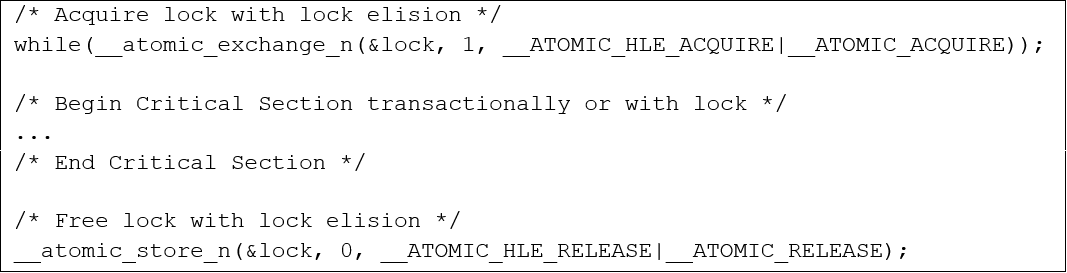
\includegraphics[width=\textwidth,height=\textheight,keepaspectratio]{fig_hleInterface}
    \caption{\textbf{Generic HLE Software Interface}}
    \label{fig:hle_interface}
\end{figure}

\indent
HLE is legacy compatible.  Code utilizing the HLE interface can be executed on
legacy hardware, but the HLE prefixes will be ignored \cite{intel_prog_ref},
i.e. the processor will always perform the write operation on the locking
variable and execute the critical section non-transactionally.  While this
interface does nothing for multi-threaded applications on legacy hardware, it
does allow for easier cross-platform code deployment.
\par

\subsubsection{\textbf{Restricted Transactional Memory (RTM)}}

\indent 
The Restricted Transactional Memory (RTM) interface introduces four new
instructions: 1) XBEGIN, 2) XEND, 3) XABORT, and 4) XTEST.  XBEGIN marks the
start of a transaction, while XEND makes the end of a transaction.  XABORT is
used by the programmer to manually abort a transaction.  XTEST can be used to
test if the processor is executing transactionally or non-transactionally.
\par

\indent 
The XBEGIN instruction transitions the processor into transactional
execution \cite{intel_prog_ref}.  Note that the xbegin instruction does not even
read the locking variable as HLE does.  Therefore, the programmer should
manually add the locking variable to the transaction's read-set by checking if
the lock is free at the start of the transaction.  If it is free, the
transaction can execute safely.  Once execution reaches the XEND instruction,
the processor will attempt to atomically commit the transaction.
\par

\indent
As previously mentioned, the transaction can abort for many reasons.
One case specific to RTM occurs when the lock is not free upon entering the
transaction.  In this case, the programmer uses the XABORT instruction to
explicitly abort the transaction.  But no matter the reason for the abort,
execution jumps to the fallback instruction address \cite{intel_prog_ref}.  This
address is an operand of the XBEGIN instruction.
\par

\indent
It is this fallback path that makes RTM a much more flexible interface
than HLE because it is entirely at the discretion of the programmer.  Even so,
the programmer must still provide an abort path that guarantees forward progress
\cite{intel_prog_ref}.  Therefore, the abort parth should use explicit
synchronization, e.g. acquire the lock, to ensure forward progress. However, the
programmer can use this abort path to tune the performance of RTM enabled
applications.  For instance, a retry routine can be used to specify how many
times the processor should attempt to enter transactional execution before using
explicit synchronization.  Furthermore, the EAX register reports information
about the condition of an abort \cite{intel_prog_ref}, such as whether or not
the abort was caused by the XABORT instruction, a data conflict, etc.  The
programmer can use this information to make more informed decisions regarding
reattempting transactional execution.
\par

\indent 
The general algorithm for the RTM software interface is shown in Figure
~\ref{fig:rtm_interface}.  The programmer moves the existing locking mechanism
inside an else clause of the xbegin if statement, which will determine if the
processor transitions to transactional execution or takes the abort path.  As
previously mentioned, the processor will also return to this point should the
transaction abort in the middle of execution. Moving the locking mechanism into
the RTM abort path ensures that the abort path ultimiately uses explicit
synchronization and guarantees forward progress.  GCC 4.8 and above includes
support for the \_xbegin, \_xabort, and \_xend intrinsics \cite{gcc}.

\begin{figure}[H]
    \centering
    \graphicspath{ {./figures/} }
    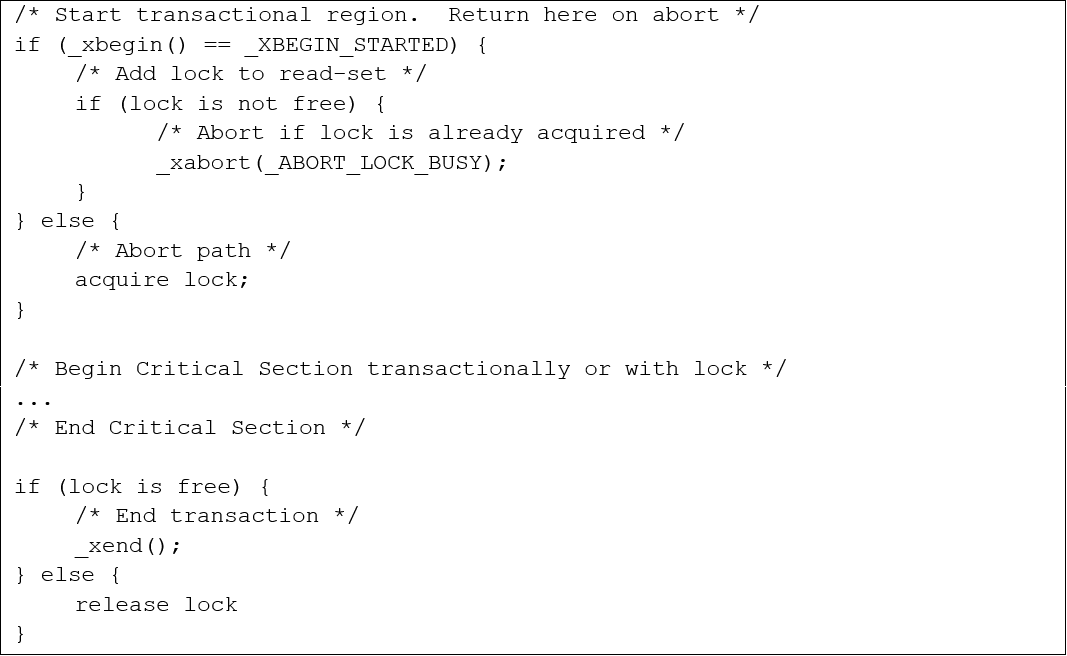
\includegraphics[width=\textwidth,height=\textheight,keepaspectratio]{fig_rtmInterface}
    \caption{\textbf{Generic RTM Software Interface}}
    \label{fig:rtm_interface}
\end{figure}

\indent 
While RTM is a much more flexible interface than HLE, it can only be
used on supported Haswell platforms.  If a legacy device attemps to execute one
of the RTM instructions, it will throw a General Protection Fault.  It should
be noted that execution of the XEND instruction outside of a transaction
will result in a General Protection Fault as well \cite{intel_opt_man}.
\par

\newpage
\section{\textbf{Practical Programming with TSX}}

\indent 
One of the disadvantages of HTM is the physical limitations of the
hardware.  This section evaluates practical programming techniques to consider
when using TSX to ensure optimal performance.  Custom benchmarks were developed
to evaluate these various constraints.  All benchmarks were run on a system with
an Intel i7-4770 running at 3.4GHz with 32 GB RAM.  Each core has a 32KB 8-way,
set associative L1 cache and a 256 L2 cache.  Each cache line is 64 bytes.  This
information was verified using common Unix commands.
\par

\subsection{\textbf{Memory Organization}}

\indent 
TSX maintains a read-set and a write-set with the granularity of a cache line
\cite{intel_prog_man}.  During transactional execution, TSX constructs a
record of memory addresses read from and a record of memory addresses written
to.  A data conflict occurs if another thread tries to read an address in the
write-set or tries to write an address in the read-set.  This definition can be
expanded to state that \textit{a data conflict occurs if: 1) another thread attempts to
read a memory address that occupies the same cache line as a memory address to
be written, or 2) another thread attempts to write a memory address that
occupies the same cache line as a memory address that has been read from.}
\par

\indent 
Therefore, aborts can be caused by data occupying the same cache line,
especially false sharing, i.e. the occupation of the same cache line by
unrelated data \cite{intel_opt_man}.  To mitigate the effects of shared
cache line data conflicts, the programmer must be conscientious of how data is
organized in memory.  For instance, the data in the previously discussed
benchmarks is optimally organized by allocating individual elements to 64 bytes,
i.e. a single cache line.
\par

\indent 
Furthermore, data elements should be aligned to cache line boundaries
to ensure that each element is limited to exactly one cache line.  If a data
element crosses a cache line boundary, the probability of shared cache line data
conflicts increases as the data access now has to check against two cache lines.  
\par

\subsection{\textbf{Transaction Size}}

\indent
TSX maintains a transaction read-set and write-set in the L1 cache
\cite{intel_opt_man}.  The size of these memory sets is therefore limited by
the size of the L1 cache.  Hyper-threading further restricts the size of the
transaction data sets becase the L1 cache is shared between two threads on the
same core \cite{intel_opt_man}.  Based on granularity of the read-set and write-set stated
above, transaction size is defined as the number of cache lines accessed within
a transaction.  
\par 

\indent
A set of benchmarks was developed to access a shared array of custom structures. Each
structure is allocated to occupy an entire cache line, i.e. 64 bytes, and
aligned to the nearest cache line boundary using the GCC align attribute.  This
ensures that memory is optimally organized as previously mentioned.  Benchmarks
were run with varying transaction sizes and number of threads.
\par

\indent
The first benchmark was run with a single thread to avoid data conflicts.  Figure
~\ref{fig:trx_size} shows the abort rate, i.e. \# aborts / \# operations, as the
number of cache lines accessed within the transaction increases.  The read-set
data points respresent strictly read operations while the write-set data points
represent strictly write opreations.
\par 

\begin{figure}[H]
    \centering
    \graphicspath{ {./figures/} }
    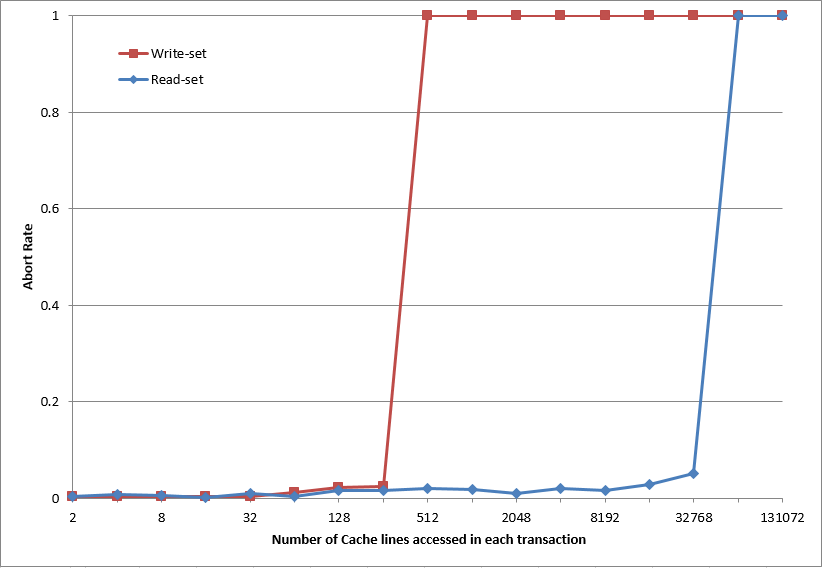
\includegraphics[totalheight=0.50\textheight,keepaspectratio]{trx_size}
    \caption{\textbf{TSX RTM abort rate versus cache lines accessed for a single
    thread on one core}}
    \label{fig:trx_size}
\end{figure}

\indent
It is clear that transactions abort 100\% of the time once the thread tries to
write to 512 or more cache lines within the transaction.  This is consistent
with the size of the L1 cache, 32KB of 64 bytes caches lines equates to 512
cache lines; it is unrealistic to expect that no other process will use the
cache while the transaction is executing and thus the transaction cannot occupy
the cache in its entirety.  Furthermore, the cache is split into 64 8-way sets;
if memory is not organized properly, the total write-set size will be reduced.
\par

\indent 
However, it is evident that the same size limitations do not hold for
the read-set size.  While eviction of a cache line containing a write-set address will
always cause a tranasctional abort, evicition of a cache line containing a
read-set address may not cause an immediate transactional abort; these cache
lines may be tracked by a second-level structure in the L2 cache
\cite{intel_opt_man}.
\par

\indent 
The second benchmark is run with two threads on the same core to
evaluate the effects of hyper-threading on TSX.  Each thread accesses the same
number of cache lines, but at different memory locations to prevent any data
conflicts. Figure ~\ref{fig:trx_size_ht} shows the abort rate for one 
of the threads as the number of cache lines accessed within each transaction
increases.
\par

\begin{figure}[H]
    \centering
    \graphicspath{ {./figures/} }
    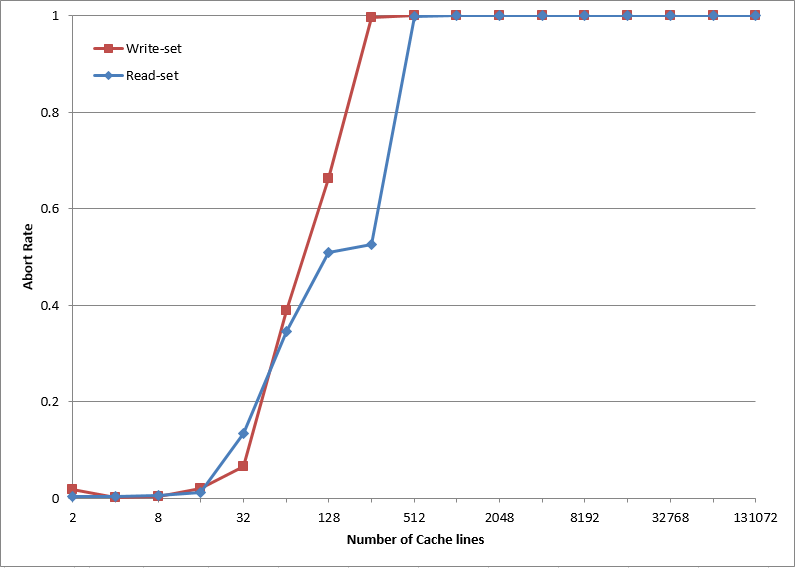
\includegraphics[width=\textwidth,height=\textheight,keepaspectratio]{trx_size_ht}
    \caption{\textbf{TSX RTM abort rate versus cache lines accessed for a two 
    threads on hyper-threaded core}}
    \label{fig:trx_size_ht}
\end{figure}

\indent 
It is evident that the write-set is strictly limited to half of the L1
cache.  However, the probability of an abort is non-trivial for any write-set
size between 32 and 128 cache lines.  It is also evident that the read-set size
is limited to a similar size as the write-set on a hyper-threaded core.
\par

\subsection{\textbf{Transaction Duration}}

\indent 
Transaction aborts can be caused by a number of run-time events
\cite{intel_prog_ref}, including but not limited to: interrupts, page faults,
I/O operations, context switches, illegal instructions, etc.  This is due to the
inability of the processor to save the transactional state information
\cite{schwahn}.
\par

\indent
To evaluate how long a transaction can safely execute for, a third
benchmark was developed to perform 100 to 1000000 increment operations on a
single element.  This benchmark was executed with a single thread to minimize
the possibility of data conflicts. Figure ~\ref{fig:trx_duration} shows the
transaction abort rate as the duration of the transaction is increased, i.e. the
number of operations performed within the transaction.
\par

\begin{figure}[H]
    \centering
    \graphicspath{ {./figures/} }
    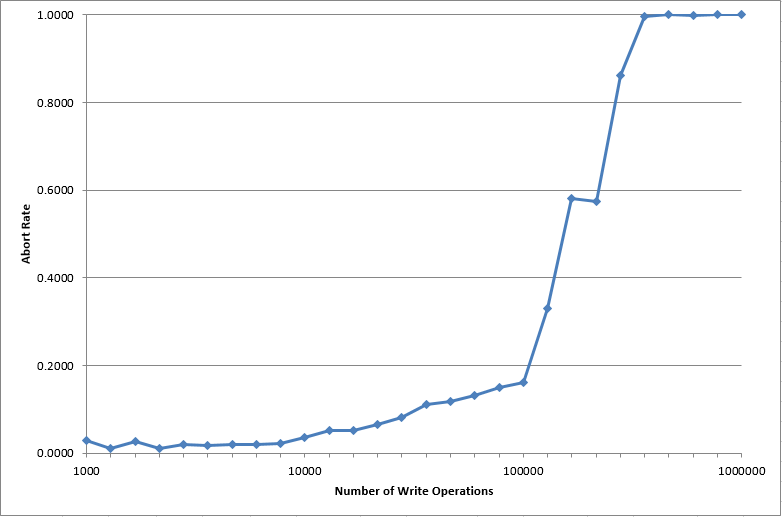
\includegraphics[width=\textwidth,height=\textheight,keepaspectratio]{trx_duration}
    \caption{\textbf{TSX RTM abort rate versus cache lines accessed for a two 
    threads on hyper-threaded core}}
    \label{fig:trx_duration}
\end{figure}

\indent 
It is clear that the longer a transaction executes, the higher the probability
is that it will abort.  Practical applications will perform a varying number of
operations that take varying amounts of time.  This benchmark simply
demonstrates that shorter transactions are more likely to succeed than longer
transactions.
\par

\subsection{\textbf{Nesting Transactions}}

\indent
When developing larger TSX enabled multi-threaded applications, it is
possible for critical sections to be nested within one another.  TSX supports
nested transactions for both HLE and RTM regions, as well as a combination of
the two.  When the processor encounters an XACQUIRE instruction prefix or an 
XBEGIN instruction, it increments a nesting count.  Note that the processor
transitions to transactional execution when the nesting count goes from 0 to 1
\cite{intel_prog_ref}.  When the processor encounters an XRELEASE instruction
prefix or an XEND instruction, the nesting count is decremented.  Once the
nesting count returns to 0, the processor attempts to commit the transactions as
one monolithic transaction \cite{intel_prog_ref}.
\par

\indent
The total nesting depth is still limited by the physical resources of
the hardware.  If the nesting count exceeds this implementation specific limit,
the transaction may abort.  Upon abort, the processor transitions to
non-transactional execution as if the first lock instruction was executed
without elision \cite{intel_prog_ref}.
\par

\indent
Scenarios may arise where different locks may be nested within the same
critical section.  For instance, one critical section may reside within a
separate critical section.  While this is not a concern for RTM regions, it can
become a concern for HLE regions, as the processor can only track a fixed number
of HLE prefixed locks.  However, any HLE prefixed locks executed after this
implementation specific limit has been reached will simply execute without
elision; consequently, the secondary lock variable will be added to the
transaction's write-set \cite{intel_prog_ref}.
\par

\newpage
\section{\textbf{Parallel Discrete Event Simulation (PDES) and WARPED}}

\indent
Parallel Discrete Event Simulation (PDES) is the simulation of a collection of
logical processes (LPs), each representing physical processes of a physical
system.  Each LP executes and generates events; upon execution of an event, the
LP updates its state and generates 0 or more events \cite{muthalagu}.  LPs are
executed concurrently, i.e. their events of are executed concurrently.  However,
events must be retrieved from a global pending event set by one of multiple
execution threads.  This process is implementation specific and will be
discussed further below.
\par

\subsection{\textbf{WARPED and the Pending Event Set}}

\indent
WARPED is a publicly available Discrete Event Simulation (DES) kernel
implementing the Time Warp protocol \cite{martin,fujimoto}.  It was recently
redesigned for parallel execution on multi-core processing nodes
\cite{muthalagu}.  It has many configuration options and utilizes many different
algorithms of the Time Warp protocol \cite{fujimoto}, many of which are beyond
the scope of this research.
\par

\indent
In WARPED, logical processes (LPs) consist of \textit{N} simulation objects.
When a worker thread removes the top event of the LTSF queue for execution, it
"schedules" the simulation object associated with that event.  To avoid
contention for objects at the LTSF queue, the worker thread removes scheduled
object from the LTSF queue to avoid multiple threads scheduling the same
simulation object \cite{muthalagu}.
\par

\indent 
The pending event set is a set of generated events that have not been
processed yet.  Its design and implementation are crucial to the performance of
the simulation \cite{twpes}.  In PDES,  

\indent
WARPED implements the pending event set in a two-level structure. Each LP
maintains its own pending event list as an independently locked list.  A common
Least Time Stamped First (LTSF) pending event queue is populated with the lowest
timestamped event from each LP's event list.  The worker threads schedule the
next events for execution from this LTSF queue, which is locked and sorted.
Clearly this results in contention between the worker threads.  Previous studies
have shown that contention for the LTSF queue negatively impacts performance
once the number of worker threads exceeds 5-6.


\subsection{\textbf{Previous Studies with the Pending Event Set in Warped}}

\indent Dickman et al. explored the explored the use of various data structures
in the WARPED pending event set implementation, specifically, the STL multiset,
splay tree, and ladder queue data structures. Furthermore, they explored the use
of multiple LTSF queues \cite{dickman}.  They found that using the ladder queue
data structure and multiple LTSF queues resulted in better simulation
performance for certain scenarios.  A secondary focus of this study will expand
upon the use of multiple LTSF queues, as well as the use of splay tree versus 
STL multiset data structures.\par

\newpage
\section{\textbf{Experimental Analysis}}

\indent This study compares the performance of the WARPED simulation kernel
using conventional synchronization mechanisms, Hardware Lock Elision, and
Restricted Transactional memory.  All simulations were performed on a system
with an Intel i7-4770 running at 3.4 GHz with 32GB of RAM.  Average execution
time and standard deviation were calculated from a set of 10 trials for each
simulation configuration.\par

\indent The simulation model used to obtain the following results is an epidemic
model.  It consists of 110998 geographically distributed people
requiring a total of 110998 LPs.  The epidemic is modeled by reaction processes
to model progression of the disease within an individual entity, and diffusion
processes to model transmission of the disease among individual entities.\par

%\subsection{\textbf{Lock Contention with Conventional Synchronization
%Mechanisms}}
%
%\indent The first part of this study benchmarked the performance of the WARPED
%simulation kernel simulating the epidemic model with the appropriate
%configuration parameters using conventional synchronziation mechanisms, i.e.
%atomic locks.  It should be noted that the original implementation of the WARPED
%pending event set only allows for a number of worker threads that is eveny
%divisble by the number of worker threads due to the way in which LP's are
%partitioned to LTSF queues.\par

\subsection{\textbf{Lock Contention}}

\indent
The first part of this study compares the performance of the original WARPED
pending event set implementation using: 1) atomic locks, 2) HLE, and 3) RTM with
1 retry, 4) RTM with 4 retries, and 5) RTM with 9 retries.  It should be noted
that the original implementation of the WARPED pending event set only allows for
a number of worker threads that is eveny divisble by the number of worker
threads due to the way in which LP's are partitioned to LTSF queues.  These
results are shown in Figures ~\ref{fig:noThrMig_timeVSthreads_1schq} and Tables
~\ref{tab:noThrMig_2threadsXschq}, ~\ref{tab:noThrMig_4threadsXschq}, and
~\ref{tab:noThrMig_6threadsXschq}.\par

\begin{figure}[H]
    \centering
    \graphicspath{ {./figures/} }
    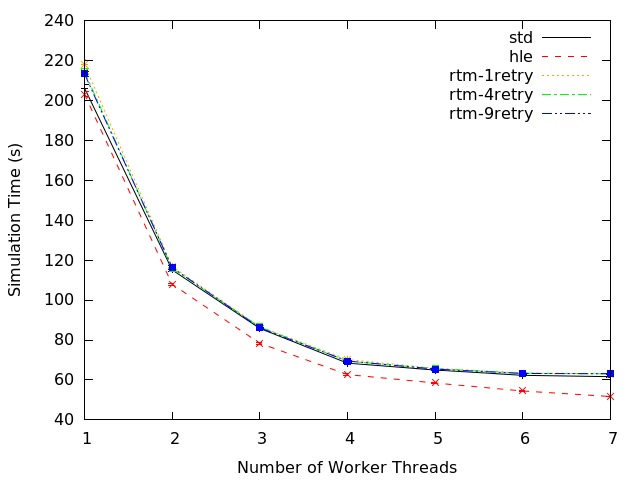
\includegraphics[width=\textwidth,height=\textheight,keepaspectratio]{noThrMig-summary-multiset-hugeepidemicsim-timeVSthreads-1schQ}
    \caption{\textbf{Simulation Time as Number of Worker Threads is Increased
    Using Various Synchronization Mechanisms for 1 STL Multiset LTSF Queue}}
    \label{fig:noThrMig_timeVSthreads_1schq}
\end{figure}

\begin{table}[H]
    \centering
    \begin{tabular}{l|p{2cm}|p{2cm}|p{2cm}|p{2cm}|p{2cm}}
        \textbf{\# LTSF Queues}&Lock &HLE &RTM 1-retry &RTM 4-retry &RTM-9retry \\
        \hline
        \midrule
            1 &115.1073 &107.93   &116.8573 &115.8511 &116.3141 \\ 
            2 &111.6427 &104.7166 &113.0621 &121.884  &130.4556   
    \end{tabular}
    \caption{\textbf{Simulation Times for 2 Worker Threads with X LTSF Queues}}
    \label{tab:noThrMig_2threadsXschq}
\end{table}

\begin{table}[H]
    \centering
    \begin{tabular}{l|p{2cm}|p{2cm}|p{2cm}|p{2cm}|p{2cm}}
        \textbf{\# LTSF Queues}&Lock &HLE &RTM 1-retry &RTM 4-retry &RTM-9retry \\
        \hline
        \midrule
            1 &68.40767  &62.70367 &70.23204  &69.44761 &69.46226 \\ 
            2 &73.62335  &69.23382 &74.28421  &74.5701  &74.40304 \\
            4 &100.74668 &97.87896 &100.70637 &98.65185 &97.00871 
    \end{tabular}
    \caption{\textbf{Simulation Times for 4 Worker Threads with X LTSF Queues}}
    \label{tab:noThrMig_6threadsXschq}
\end{table}

\begin{table}[H]
    \centering
    \begin{tabular}{l|p{2cm}|p{2cm}|p{2cm}|p{2cm}|p{2cm}}
        \textbf{\# LTSF Queues}&Lock &HLE &RTM 1-retry &RTM 4-retry &RTM-9retry \\
        \hline
        \midrule
            1 &62.32475 &54.4856  &63.46503 &63.38292 &63.22529 \\  
            2 &61.03439 &56.03277 &61.72473 &61.38556 &61.23396 \\  
            3 &65.605   &63.3307  &65.24451 &64.92354 &64.93433 \\  
            6 &73.50022 &69.54849 &72.83046 &71.01408 &64.13042   
    \end{tabular}
    \caption{\textbf{Simulation Times for 6 Worker Threads with X LTSF Queues}}
    \label{tab:noThrMig_6threadsXschq}
\end{table}

\indent
It is evident from Figure ~\ref{fig:noThrMig_timeVSthreads_1schq} that
contention is increasing as the number of worker threads increases.
Furthermore, it would appear that utilizing more than one LTSF queue is no
longer producing consistent or desirable results. It was also observed that the
number of rollbacks was non-trivial for these simulations.  These poor
performance could be attributed to recent changes made to the WARPED kernel.\par

\subsubsection{\textbf{Continuous Thread Migration}}

\indent
Based on the less than desirable results above, a roaming thread migration
technique was implemented to alleviate contention on the LTSF queues.  It
distributes threads that attempt to access the same LTSF queue to separate LTSF
queues.  Pseudocode for this implementation can be seen in Figure
~\ref{fig:thread_migration} \(\textbf{TODO:get psuedocode figure}\).  Many
details are omitted for clarity.\par

\begin{figure}[H]
    \centering
    \graphicspath{ {./data/} }
    \caption{\textbf{Generalized event execution loop for migration worker
    threads}}
    \label{fig:thread_migration}
\end{figure}

\subsubsection{\textbf{Thread Migration for X Events}}

\newpage
\section{\textbf{Conclusions}}






%    \begin{figure}[H]
%        \centering
%        \includegraphics[width=\textwidth,height=\textheight,keepaspectratio]{../../magic/pics/magic_layout_32_bit.png}
%        \caption{\textbf{32 Bit Layout - Magic}}
%        \label{fig:gg}
%    \end{figure}

%\section{\textbf{Work Division}}
%    \begin{table}[H]
%        \centering
%        \begin{tabular}{l | p{8cm}}
%            \hline
%            \textbf{Student}   & \textbf{Task} \\ \hline
%            \midrule
%                Both        & Modified Pin-out Diagram \\
%                Both        & Magic Layout \\
%                Both        & IRSIM \\
%                Both        & VHDL \\
%                Both        & Modified Floor Plan
%        \end{tabular}
%        \caption{\textbf{Task Assignment}}
%    \end{table}

\newpage
\bibliographystyle{abbrv}
\bibliography{refs}

\end{document}
